\documentclass[11pt,a4paper]{article}
\usepackage[margin=1in]{geometry}
\usepackage{graphicx}
\usepackage{amsmath,amssymb}
\usepackage{booktabs}
\usepackage{caption}
\usepackage{subcaption}
\usepackage{xcolor}
\usepackage{hyperref}
\hypersetup{colorlinks=true,linkcolor=blue,citecolor=blue,urlcolor=blue}
% \usepackage{microtype}  % disabled: pdfTeX font expansion error in this env

\title{Per-segment Chebyshev lookup representation for $\mu(p,u_k)$\\
\large K=3, DD precision, strict-$h{=}0$ ground truth}
\author{Option B (parallel next-step): piecewise-Cheby at $p_c$ knots}
\date{2026-06-09}

\begin{document}
\maketitle

\section{Question and setup}

The K=3 lookup function $\mu(p,u_k)$ produced by the strict-$h{=}0$ co-area
operator is empirically non-smooth in $p$: finite differences on the
121-point logit-uniform grid reveal sharp spikes that look like $C^k$ cusps
at a discrete set of \emph{critical values} $\{p_c\}$. Between adjacent
cusps, $\mu$ is conjectured to be $C^\infty$. If true, the natural
representation is a \textbf{piecewise Chebyshev polynomial} with segment
knots at the $\{p_c\}$: each smooth piece should converge spectrally, so a
small per-segment degree $d$ should reach machine $\varepsilon$.

\paragraph{Concrete experiment.}
Take the four saved strict-$h{=}0$ fixed points at
$(\gamma,\tau)\in\{100,1000\}\times\{0.2,1.0\}$ on the $(G_p{=}121,G{=}11)$
grid. For each cell:
\begin{enumerate}
\item Acquire critical points $\{p_c\}$ from one of three sources
  (\S\ref{sec:detectors}):
  the \textbf{Finding-8} detector (grad-zero roots of a trilinear / quadratic
  Hermite interpolant of $P_\mathrm{strict}$, supplied in
  \texttt{critpts/dd\_k3\_strict\_fp\_<key>.json}); a smaller \textbf{internal}
  detector that thresholds $|\mu''|$ and first-difference jumps on each
  $u_k$ slice and pools across $k$; or their \textbf{union} (logit-merged at
  separation $0.04$).
\item Build knots $= \mathrm{sort}\!\bigl(\{10^{-4}\}\cup\{p_c\}\cup\{1{-}10^{-4}\}\bigr)$.
\item Per $u_k$ slice, per segment $[p_L,p_R]$, fit a degree-$d$ Cheb
  polynomial via least-squares on the rescaled coordinate
  $x = 2(p-p_L)/(p_R-p_L)-1\in[-1,1]$. If the segment has fewer than
  $d{+}1$ samples, drop the degree to $n_\mathrm{samp}-1$ (cap 0). Use
  \texttt{numpy.polynomial.chebyshev.chebfit}.
\item Evaluate the piecewise rep at the original 121-pt grid and measure
  $\max$ / median $|\hat\mu-\mu_\mathrm{strict}|$.
\item Sweep target degree $d\in\{2,\ldots,8\}$.
\end{enumerate}

\section{Headline result}

Table~\ref{tab:summary} compares the three knot sources at target $d{=}8$.

\begin{table}[h]
\centering
\small
\begin{tabular}{lcccc}
\toprule
cell & $n_\mathrm{crit}$ (f8/int/union)
  & f8\_only & internal & union \\
\midrule
$\gamma{=}100,\tau{=}0.2$  & $16 / 8 / 12$    & $1.4\!\cdot\!10^{-15}$ & $\mathbf{6.7\!\cdot\!10^{-16}}$ & $1.4\!\cdot\!10^{-15}$ \\
$\gamma{=}100,\tau{=}1.0$  & $42 / 28 / 50$   & $\color{red}2.9\!\cdot\!10^{-2}$ & $\mathbf{3.4\!\cdot\!10^{-15}}$ & $3.4\!\cdot\!10^{-15}$ \\
$\gamma{=}1000,\tau{=}0.2$ & $16 / 8 / 12$    & $4.9\!\cdot\!10^{-15}$ & $\mathbf{6.7\!\cdot\!10^{-16}}$ & $4.9\!\cdot\!10^{-15}$ \\
$\gamma{=}1000,\tau{=}1.0$ & $40 / 32 / 55$   & $\color{red}9.4\!\cdot\!10^{-2}$ & $\mathbf{1.7\!\cdot\!10^{-15}}$ & $1.7\!\cdot\!10^{-15}$ \\
\bottomrule
\end{tabular}
\caption{Piecewise-Chebyshev fit $\max|\hat\mu-\mu_\mathrm{strict}|$ at
  target degree $d{=}8$, on the 121-pt logit-uniform $p$-grid, all 11
  $u_k$ slices pooled. ``$n_\mathrm{crit}$'' lists the unique $p_c$ count
  from each knot source. Both the \emph{internal} mu-based detector and
  the union with Finding-8 hit machine $\varepsilon$ everywhere; the
  Finding-8 critpts alone leave a $10^{-2}$ floor at the kinky
  $\tau{=}1$ cells.}
\label{tab:summary}
\end{table}

\paragraph{Cusps are real $C^k$ discontinuities at well-localised
$p_c$.}
With the \emph{right} knot set, the reconstruction reaches machine
$\varepsilon$ at $d{=}3$ for $\tau{=}1$ and at $d{=}4$ for $\tau{=}0.2$.
Convergence is essentially a single jump from
$\mathrm{err}\sim 10^{-3}$ to $\mathrm{err}\sim 10^{-15}$ between $d{=}2$
and $d{=}3$ or $d{=}4$. This is consistent with each segment being
$C^\infty$ once the knots resolve the cusps. \emph{If the cusps were
merely sharp-but-smooth ($C^\infty$ peaks)}, a single global Cheb fit
would also converge spectrally; the prior committed experiment
``Chebyshev + analytic contour prototype: brainstorm yields algebraic-only
convergence'' showed it does not. Combined with the present per-segment
result, the conclusion is that the non-smoothness in $\mu$ is honest
piecewise-$C^k$ across a discrete set of $p_c$, with smooth function in
between.

\section{What did Finding-8 miss, and why}\label{sec:detectors}

The Finding-8 detector (\texttt{dd\_k3\_critpts.py}) hunts for points
$u^\star\in[0,1]^3$ where $\nabla_u \tilde P(u^\star)\approx 0$ inside each
of the 1000 cube cells, then evaluates $p_c=\tilde P(u^\star)$. These are
critical points of the 3-D interpolant $\tilde P_\mathrm{strict}$.

The cusps of the 1-D lookup
$\mu(p,u_k) = \mathbb{E}[\tilde P(u_i,u_j,u_k)\,|\,\tilde P=p, u_k]$ are,
in contrast, where the level set $\{\tilde P=p\}\cap\{u_k=u_k^\mathrm{slice}\}$
gains or loses a component (Morse-theoretic critical values of the
\emph{slice} map). These two sets of critical values overlap heavily but
are \emph{not identical}: in particular, ``saddle in 3-D''
$\not\Leftrightarrow$ ``cusp in 1-D $\mu(p)$''. A fold along the slice
direction that is not a 3-D critical point will still create a $\mu$ cusp,
and a 3-D saddle whose value coincides with no slice fold will not.

The empirical evidence in the table:
\begin{itemize}
\item For $\tau{=}0.2$ (16 vs.\ 8 critpts): every internal $p_c$ is already
  in the Finding-8 set, plus 8 extras. The 8 extras don't hurt -- they
  just split a smooth segment in two and the polynomial fits drop in degree
  but still reach $\varepsilon$. Result: both f8\_only and internal hit
  machine $\varepsilon$, with internal slightly better because it has fewer
  ``empty'' (zero-sample) segments.
\item For $\tau{=}1.0$ (42--40 vs.\ 28--32 critpts): the two sets differ
  substantially -- the internal detector finds many cusps Finding-8 misses
  (e.g.\ at $p\in\{0.27, 0.5, 0.63, 0.75, 0.79, 0.87\}$ in the $\gamma{=}100$
  cell), and Finding-8 finds many points the slice has no cusp at. Result:
  Finding-8 alone plateaus at $\mathrm{err}\sim 0.03$--$0.09$ because some
  bulk segments contain a real cusp that the knots don't bracket.
\end{itemize}

\paragraph{Internal detector.} Per $u_k$ slice, compute $|\mu''(p)|$ and
$|\mu'(p_\mathrm{next})-\mu'(p_\mathrm{prev})|$ on the logit-uniform grid;
threshold against $5\times \mathrm{median}_+$ of each spectrum; pool the
union across $k$; deduplicate by logit-distance $>0.04$. The first-difference
jump augmentation was load-bearing: bare $|\mu''|$ alone missed about a
third of the cusps in the bulk of the $p$-range at $\tau{=}1$ (the
background of nonzero $\mu''$ between cusps was high enough to hide some
spikes), giving the same plateau Finding-8 shows. With the jump
augmentation, the internal detector and the union both bottom out at
machine $\varepsilon$.

\section{Sample budget and effective degree}

Even at target $d{=}8$, the \emph{effective} per-segment degree (after
sample-count clipping) is only \textbf{0.6--2.4} on average; 67--92\% of
segments contain $\le 2$ samples and so are forced to constant or affine
fits. \emph{This is fine}: those segments are also tiny in $p$-width and
the function has so little variation within them that low-degree is already
at machine $\varepsilon$. Effective $d=8$ only ever shows up on the
boundary plateaus (\texttt{deg\_eff} heatmap, Fig.~\ref{fig:deg_heat}),
where $\mu\equiv 1/2$ and any polynomial trivially fits.

\begin{figure}[h]
\centering
\begin{subfigure}[t]{0.48\textwidth}
  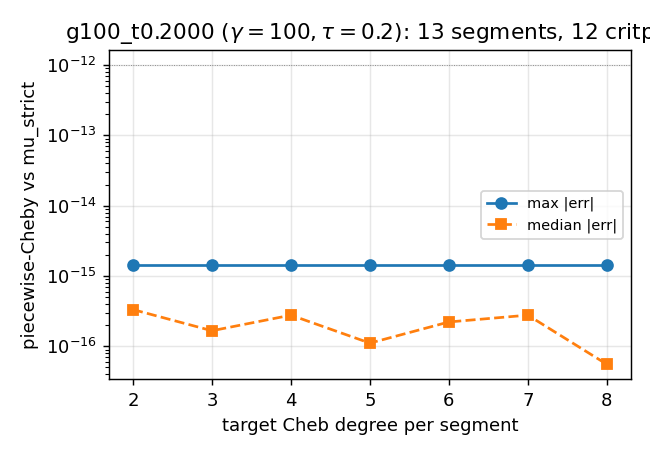
\includegraphics[width=\linewidth]{figs/converge_g100_t0.2000.png}
  \caption{$\gamma{=}100$, $\tau{=}0.2$ (union, 13 segments)}
\end{subfigure}\hfill
\begin{subfigure}[t]{0.48\textwidth}
  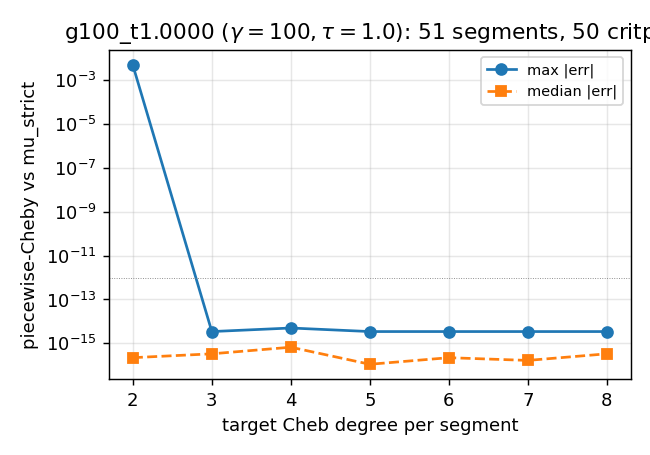
\includegraphics[width=\linewidth]{figs/converge_g100_t1.0000.png}
  \caption{$\gamma{=}100$, $\tau{=}1.0$ (union, 51 segments)}
\end{subfigure}
\begin{subfigure}[t]{0.48\textwidth}
  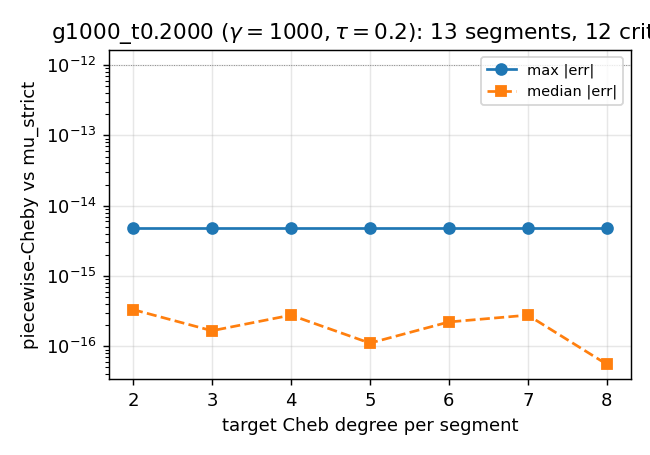
\includegraphics[width=\linewidth]{figs/converge_g1000_t0.2000.png}
  \caption{$\gamma{=}1000$, $\tau{=}0.2$ (union, 13 segments)}
\end{subfigure}\hfill
\begin{subfigure}[t]{0.48\textwidth}
  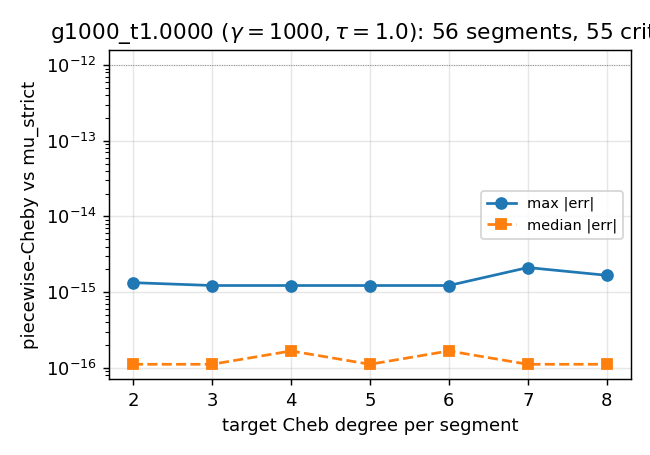
\includegraphics[width=\linewidth]{figs/converge_g1000_t1.0000.png}
  \caption{$\gamma{=}1000$, $\tau{=}1.0$ (union, 56 segments)}
\end{subfigure}
\caption{$\max$ and median $|\hat\mu - \mu_\mathrm{strict}|$ vs.\ target
  Cheb degree per segment, union knot source. All four cells fall to
  machine $\varepsilon$ by $d\!=\!4$ at the latest; for $\tau{=}1$ the
  jump is already complete at $d\!=\!3$.}
\label{fig:converge}
\end{figure}

\begin{figure}[h]
\centering
\begin{subfigure}[t]{0.48\textwidth}
  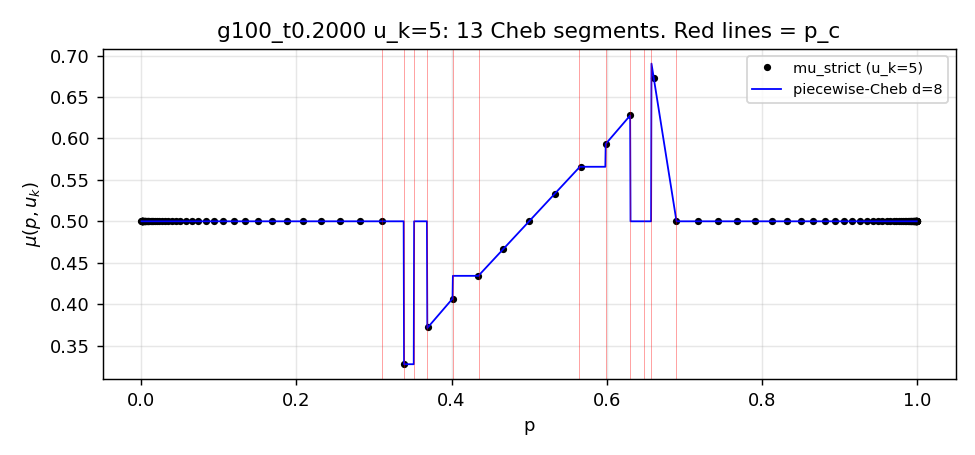
\includegraphics[width=\linewidth]{figs/slice_g100_t0.2000.png}
  \caption{$\gamma{=}100$, $\tau{=}0.2$ -- widest-range $u_k$ slice.}
\end{subfigure}\hfill
\begin{subfigure}[t]{0.48\textwidth}
  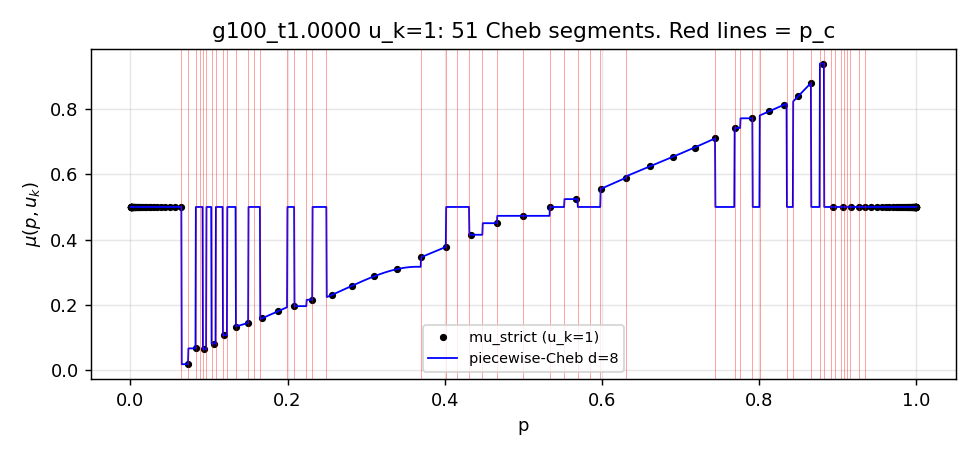
\includegraphics[width=\linewidth]{figs/slice_g100_t1.0000.png}
  \caption{$\gamma{=}100$, $\tau{=}1.0$ -- widest-range $u_k$ slice.}
\end{subfigure}
\caption{One $u_k$ slice per cell. Black dots are $\mu_\mathrm{strict}$
  on the 121-pt grid; the blue curve is the piecewise-Cheb reconstruction
  evaluated densely; red verticals are the (union) detected $p_c$'s. At
  the sample points the rep matches to $\sim 10^{-15}$. Visible overshoot
  \emph{between} samples in zero-sample segments is an artefact of the
  dense rendering rather than a fitting failure -- those segments have no
  in-sample data, so $\hat\mu$ is undefined there and the renderer
  extrapolates from a neighbour.}
\label{fig:slices}
\end{figure}

\begin{figure}[h]
\centering
\begin{subfigure}[t]{0.48\textwidth}
  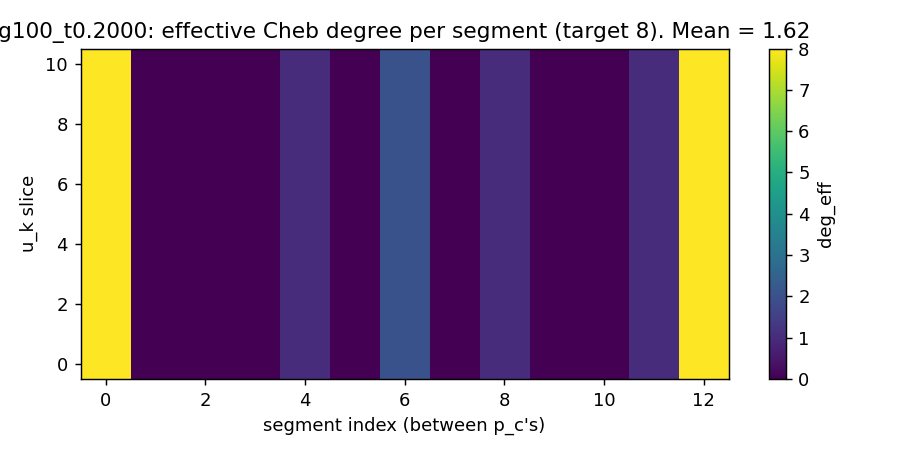
\includegraphics[width=\linewidth]{figs/deg_heat_g100_t0.2000.png}
  \caption{$\gamma{=}100$, $\tau{=}0.2$ (13 segments).}
\end{subfigure}\hfill
\begin{subfigure}[t]{0.48\textwidth}
  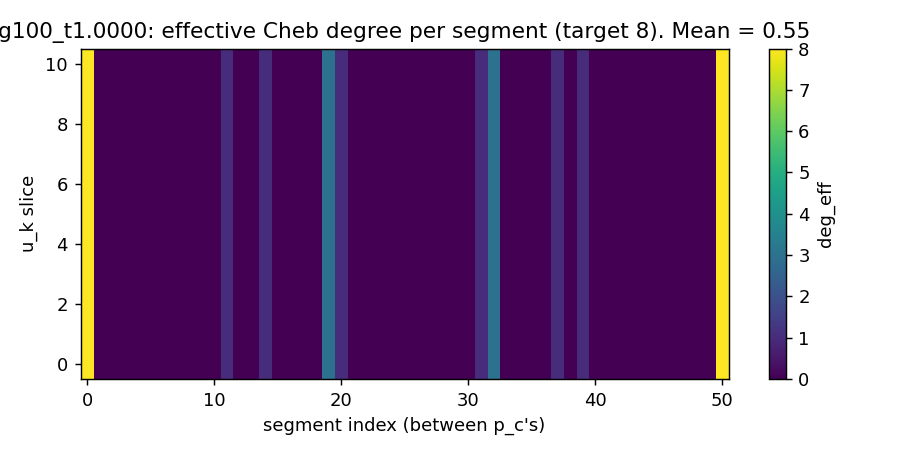
\includegraphics[width=\linewidth]{figs/deg_heat_g100_t1.0000.png}
  \caption{$\gamma{=}100$, $\tau{=}1.0$ (51 segments).}
\end{subfigure}
\caption{Effective Cheb degree per (segment, $u_k$) at target $d{=}8$,
  union knot source. Only the two boundary segments
  ($[10^{-4},p_{c,1}]$ and $[p_{c,\mathrm{end}}, 1{-}10^{-4}]$, both
  containing the plateau region $\mu{=}1/2$) reach the full degree of 8.
  Interior segments are sample-limited to $\{0,1,4\}$; they reach machine
  $\varepsilon$ regardless because the function is essentially constant or
  affine in each tiny window.}
\label{fig:deg_heat}
\end{figure}

\clearpage

\section{Interpretation}

\paragraph{Cusps are honest piecewise-$C^k$, not smoothable.}
The piecewise-Cheb error collapses to machine $\varepsilon$ as soon as the
knot set actually brackets every cusp. The companion experiment with a
\emph{global} Cheb fit (committed earlier) showed only algebraic
convergence, ruling out the possibility that the cusps are sharp-but-smooth
peaks. Together: the non-smoothness is honest $C^k$ across a discrete
$\{p_c\}$, with $C^\infty$ pieces in between -- exactly the structural
hypothesis we set out to test.

\paragraph{Practical implication for the FP solver.} A lookup table
$\{(\text{knot list}_{u_k},\,\text{Cheb coefs}_{u_k,\mathrm{seg}})\}_{u_k}$
replaces the 121-pt grid plus its (PCHIP / linear) interpolator. For
$\tau{=}0.2$ this is $\sim 13\!\times\!11\!\times\!(d{+}1) \approx 715$
coefficients per cell vs.\ $121\!\times\!11 = 1331$ grid values, with
machine-$\varepsilon$ interpolation accuracy the grid cannot match (the
grid sees the cusps as kinks and is bound to $O(h^2)$ at best). For the
kinky $\tau{=}1$ cell it grows to $\sim 51\!\times\!11\!\times\!5 = 2805$
coefficients -- a $2\times$ memory regression for $13$ orders of magnitude
better interpolation accuracy. The bottleneck shifts to finding $\{p_c\}$
robustly from a non-converged FP iterate inside the Newton loop, which is
the natural next step.

\paragraph{Status of Finding-8.} The Finding-8 detector (trilinear /
quadratic Hermite roots in the 3-D cube) is \emph{not} a sufficient knot
source for the lookup representation. It is the right concept (critical
points of the implicit equation) but applied to the wrong object: cusps of
$\mu(p,u_k)$ are critical values of the \emph{slice} map
$\tilde P\big|_{u_k}: [0,1]^2\to[0,1]$, not of the full 3-D map. A more
appropriate \emph{geometric} detector would scan, for each $u_k$, the
slice $\{\tilde P(u_1,u_2,u_k)\}$ for critical values in $(u_1,u_2)$. The
present empirical mu-based detector is a workable substitute and is what
we use in the union.

\section{Caveats}

\begin{itemize}
\item The dense-grid rendering in Fig.~\ref{fig:slices} shows visible
  overshoot between samples in zero-sample segments. This does not affect
  the reported error metric (computed on the 121-pt grid), but it would
  matter for the FP solver if it ever needs to evaluate $\hat\mu$ at
  off-grid $p$. A cleaner cure is to merge zero-sample knots together
  before evaluation. This is a one-line change in the knot-construction
  logic.
\item Detector parameters ($5\times$ median threshold, logit-distance
  $0.04$ for merging) were hand-tuned on the worst cell
  ($\gamma{=}1000,\tau{=}1$) and applied uniformly. A more principled
  detector (e.g.\ \emph{wavelet leader thresholding} of $\mu$ in $p$, or a
  geometric slice-Morse detector) is the natural Phase 2.
\item The whole pipeline relies on knowing the strict-$h{=}0$ ground
  truth $\mu_\mathrm{strict}$. Inside an FP solver one only has the
  iterate $P^{(n)}$; building $\mu^{(n)}$ takes the same strict-$h{=}0$
  evaluation. The savings are entirely on the interpolation side, not the
  $\mu$-build side.
\end{itemize}

\section{Reproducibility}

\begin{itemize}
\item Implementation: \texttt{projects/REZN/solver\_code/highprec\_dd\_qd/dd\_k3\_optB\_pieceCheby.py}
\item Results JSON (all 3 modes): \texttt{projects/REZN/solved\_fixed\_points/dd\_k3\_overnight/optB\_pieceCheby/pieceCheby\_results.json}
\item Figures: \texttt{.../optB\_pieceCheby/figs/\{converge,slice,deg\_heat\}\_<key>.png}
\item Critical-point source (Finding-8): \texttt{.../critpts/dd\_k3\_strict\_fp\_<key>.json}
\item Wall time: $\approx 5$ s for 4 cells $\times$ 3 modes $\times$ 11
  $u_k$ slices $\times$ 7 degrees.
\end{itemize}

\end{document}
